\chapter{\added{General discussion}}

\added{
  The general discussion begins by summarizing the limitations of this doctoral study (Section~\ref{sec:reslim}). Following that, discussing the potential solutions for future research opportunities are outlined (Section~\ref{sec:respros}).
}

% \section{\replaced{Reseach limitations}{ Conclusions and reflections}} \label{sec:reslim}
\section{\added{Reseach limitations}} \label{sec:reslim}

% \deleted{This is the first study that combined the advances of aerial (high throughput) and close-range (high quality) surveys in plant phenotyping applications to field-grown crops. This Ph.D. thesis aimed to improve the performance of 3D-based plant phenotyping on field-grown broccoli as a representative of row-planted crops having harvestable organs on the top of canopy, using only low-cost \gls{rgb} cameras. Using \gls{uav} for aerial surveys and photogrammetry allows for the efficient acquisition of 2D field maps and 3D models of the crop canopy for the entire farmland. However, due to limitations in survey efficiency and wind blurring caused by propellers, the \gls{uav} cannot fly too close to plants, resulting in inadequate resolution and quality for directly analyzing the broccoli heads at the organ level. This thesis attempted to fuse the close-range and aerial 3D phenotype data, as well as some latest machine learning and deep learning techniques, to accurately and efficiently obtain the position and size of broccoli heads in the field. Furthermore, this thesis also provided a better 3D virtual visualization for those broccoli heads in the field and builds a foundation for digital twins and virtual farmland for smart agriculture.}

% cp 2-4
% \deleted{We first developed an almost automated close-range pipeline to obtain the high-quality 3D models of destructively sampled broccoli heads, as a template database. By using the dual-rotation methods and the automated rotation platform, images from different perspectives of broccoli heads for 3D reconstruction were collected without heavy labor. Two pre-trained deep learning networks were used to preprocess these images without paying too much attention to algorithm developing and training data annotation. Afterward, we developed an automated workflow to calculate the 3D-based morphological traits and correct the top direction, which ensured the 3D models of the broccoli head can be used directly for the next step.}

% \deleted{Parallel to the close-range pipeline, we also developed the aerial pipeline to obtain the 3D models of the entire field by \gls{uav} photogrammetry. The key idea is to obtain the shape and position of each broccoli head in the field. But the resolution of photogrammetry-produced field maps or 3D models is not enough for accurate head segmentation. To improve the quality and labor for head segmentation, we first fused the raw \gls{uav} images, which have better resolution and quality, and the field map, which has unique geographical coordinates. Then, we fused the time-series data from different growing stages; the seedling stage was used to obtain the position and IDs of each broccoli, which is a very simple detection task; and these positions were used to narrow the image processing area for head segmentation. Lastly, labor-saving active learning was used to interactively annotate the training data for the segmentation deep learning model. The morphological traits of segmented broccoli heads were also calculated, which is fundamental for the final step.}

% \deleted{Finally, we fused the close-range and aerial pipelines. By using the paired morphological traits data from those destructively sampled broccoli heads, we trained an \gls{automl} calibration model to further improve the accuracy of aerial head segmentation. Then, the accuracy of head center positions was also calibrated by the piecewise affine transformation. Finally, for each broccoli head from the aerial survey, the closest 3D model was matched and transformed from the close-range high-quality database. After placing those transformed 3D models back into the aerial model, a script was developed for 3D virtual visualization and a better understanding of the head growth status in the field.}

% \deleted{Overall, the results of these three research chapters showed that the proposed pipelines including active learning, deep learning, backward projection, auto machine learning, template matching, and data fusion, led to improved performance in the tested broccoli fields from 2020 to 2022. The results and statistical analysis concluded that the research objectives have been achieved and all the source codes are published on GitHub for replication and any usage purposes, we can conclude that the research has made a positive contribution to the 3D-based plant phenotyping and precision agriculture for broccoli farmlands.}

% limitations -> combine all chapters, and new points can be found?
% \deleted{Despite the promising results of the experiment in the broccoli field over three years, there is currently no strong evidence that the proposed methods can achieve similar performance in different farmland or vegetables. Since several assumptions of the methods were based on the characteristics of broccoli heads, such as the solid shape of broccoli head when vertically rotating on the rotation platform, small position variation from seeding to heading, the circular shape of the broccoli head, the clear color differences between the crown and stem for broccoli heads, and the flatten mushroom-shaped broccoli crown shape. Hence, the proposed full pipelines cannot be applied directly to vegetables with variate shapes. The full pipelines may still work on the cauliflowers (just change the color from greenish to whitish); For vegetables like sweet potatoes and cabbages with very different shapes, some modules like close-range reconstruction or 3D-based morphological traits calculation may still work, but some kinds of modifications for other parts are expected. Another limitation of the proposed close-range and aerial data fusion is the visibility of targets in both pipelines, at least for the current stage, not directly applicable for sweet potatoes and potatoes whose targets are beneath the soil, which deserve further studies.}

\added{
  Although the three-year experiment conducted in the broccoli field yielded promising outcomes, the study was also subject to certain limitations.
  This section provides a summary of three specific limitations encountered: 
  the overreliance on broccoli-specific algorithms (Subsection~\ref{sec:lackuni}), 
  the lack of real farmland testing (Subsection~\ref{sec:lackvlid}), 
  and inadequate contributions in fieldwork and data collection (Subsection~\ref{sec:lackdata}).
}

\subsection{\added{Lacking universality}} \label{sec:lackuni}

\added{
  This study relied on certain assumptions about the characteristics of broccoli heads when developing the methods and algorithms.
  However, at present, there is insufficient evidence to support the claim that the proposed methods can achieve comparable results across various farmland or plant species.
}

\added{
  In Chapter 2, an important assumption for the high-quality 3D reconstruction pipeline is that the broccoli head remains rigid and does not change when vertically rotated on the rotation platform. 
  This assumption allows for the alignment and production of good quality 3D models through \gls{sfm}-\gls{mvs} algorithms using images captured from different view angles. 
  While this assumption holds for cauliflowers, sweet potatoes, and fruits like apples and oranges, whose bodies are almost rigid, it does not hold for plants with soft stems, leaves and even roots.
  In such cases, the study proposed pipeline is not suitable, and a better solution is to utilize fixed-object methods (Figures \ref{fig:des1}a and \ref{fig:des1}b) to achieve improved results.
}

\added{
  The postprocessing algorithms for broccoli crown segmentation and rotation in this study were also developed based on the characteristics of the broccoli head.
  Specifically, the algorithm combines the distinct color differences between the crown (dark green) and stem (light green) with a 2-class clustering algorithm to separate the two parts.
  Additionally, the flattened, mushroom-shaped form of the broccoli crown is utilized to determine the normal vector in the upward direction.
  These algorithms are specifically designed for broccoli head cases and may not apply to other vegetables and fruits.
}

\added{
  In Chapter 3, the assumption of minimal positional variation in broccoli from seeding to heading is crucial. 
  In our study, we employed the results of seeding position detection to refine the image processing region during the challenging heading stage. 
  The concept of simplifying complex detection or segmentation tasks by incorporating data collected from an earlier period has also proven effective in other application scenarios. 
  For instance, \mbox{\citet{mu_characterization_2018}} successfully obtained the convex hulls of peach tree crowns during the winter season, which were then utilized to guide the demanding crown segmentation task in summer. 
  Similarly, \mbox{\citet{li_multi-source_2023}} accurately located maize positions during the seeding stage, and these positions served as a guide for the challenging segmentation tasks when the maize canopy has severe leaf overlapping. 
  However, this assumption does not apply to targets that frequently change due to wind, such as wheat and sorghum tassels. 
  it is necessary and valuable to develop different processing algorithms to address such cases in the future.
}

\added{
  We utilized EasyIDP as another valuable tool in this chapter, but it is reported to have a potential performance bottleneck. 
  EasyIDP enables the linking of the same broccoli from low-quality geo-referenced map images to high-quality non-geo-referenced raw images, thereby greatly enhancing the accuracy of head segmentation. 
  In our experiment field, which spanned just one to two hectares, no significant performance bottlenecks were observed during the data processing. 
  However, Dr. Wei Guo reported that when processing a large forest area of over 58 hectares with file sizes exceeding 23GB using EasyIDP, the process took over 3 hours. 
  This performance bottleneck needs to be solved to facilitate the widespread application of this approach in large farmlands.
}

\added{
  In Chapter 4, to fuse the high-quality head 3D model with the low-quality aerial canopy model, we assume that all broccoli heads share similar structures for the same cultivar in the same field condition. 
  This allows us to create a representative template database through proper sampling. 
  Each head can then be approximated after a simple template transformation, which involves scaling along the short and long axes and rotating to overlap. 
  Regarding the specific data fusion operation of putting the transformed template back into the field canopy, we make further simplifying assumptions: 
  1) The shape of the broccoli head is approximately circular. 
  Therefore, even if some heads are occluded by leaves in the aerial images, we can obtain the location of the center by fitting the exposed portion. 
  This allows us to determine the X and Y coordinates for placing the transformed template back. 
  2) The broccoli heads tend to grow upright. 
  As a result, the center obtained in assumption (1) represents the highest point of the broccoli crown in the vertical direction. 
  This allows us to determine the Z coordinate for placing the template back. 
  While our results demonstrate significant quality improvement for the broccoli heads after this data fusion process (refer to Figure~\ref{fig:xrs6}), it is important to note that this is merely an approximation of size and better visualization of the calibrated morphological traits. 
  It does not capture the details present in the actual field. 
  Firstly, the shape of a broccoli head is a more complex fractal shape. Additionally, when the planting density is too high, some heads may be "squeezed" and grow at a skewed angle, which contradicts the simplifying assumptions mentioned earlier. 
  Furthermore, this approach is only applicable to visible broccoli heads in the aerial images and does not work for heavily occluded or completely invisible heads. 
  Especially, this method is not suitable for other challenging crops, such as potato and sweet potato, where the harvestable parts are underground. 
  Exploring how to deal with such complex and invisible conditions, like maize canopies and potato canopies, is a valuable avenue for future research.
}

\subsection{\added{Lacking real farmland practices}} \label{sec:lackvlid}

\added{
  One unavoidable limitation of this study is that it has not been tested in actual farmlands, which are much larger and more complex than the current experimental field. 
  One noticeable difference is the variation in canopy patterns caused by different plant densities.
  For instance, our experimental field strictly maintained a spacing of 35 cm in rows and 70 cm apart, with a smaller deviation of less than 3 cm (Fig.~\ref{fig:dis_pattern}.a).
  In contrast, in the broccoli farmland we collaborated with in another project in Fukushima, the plants were spaced approximately 35 cm apart in rows, with a considerable variation greater than 7 cm (Fig.~\ref{fig:dis_pattern}.b). 
  This difference in density and deviation not only leads to distinct canopy patterns but also affects the direction and straightness of the ridges.
  The challenges posed by this difference in our proposed pipeline can be summarized in the following three points.
}

\begin{figure}[htb!]
  \begin{center}
    \resizebox{\textwidth}{!}{
      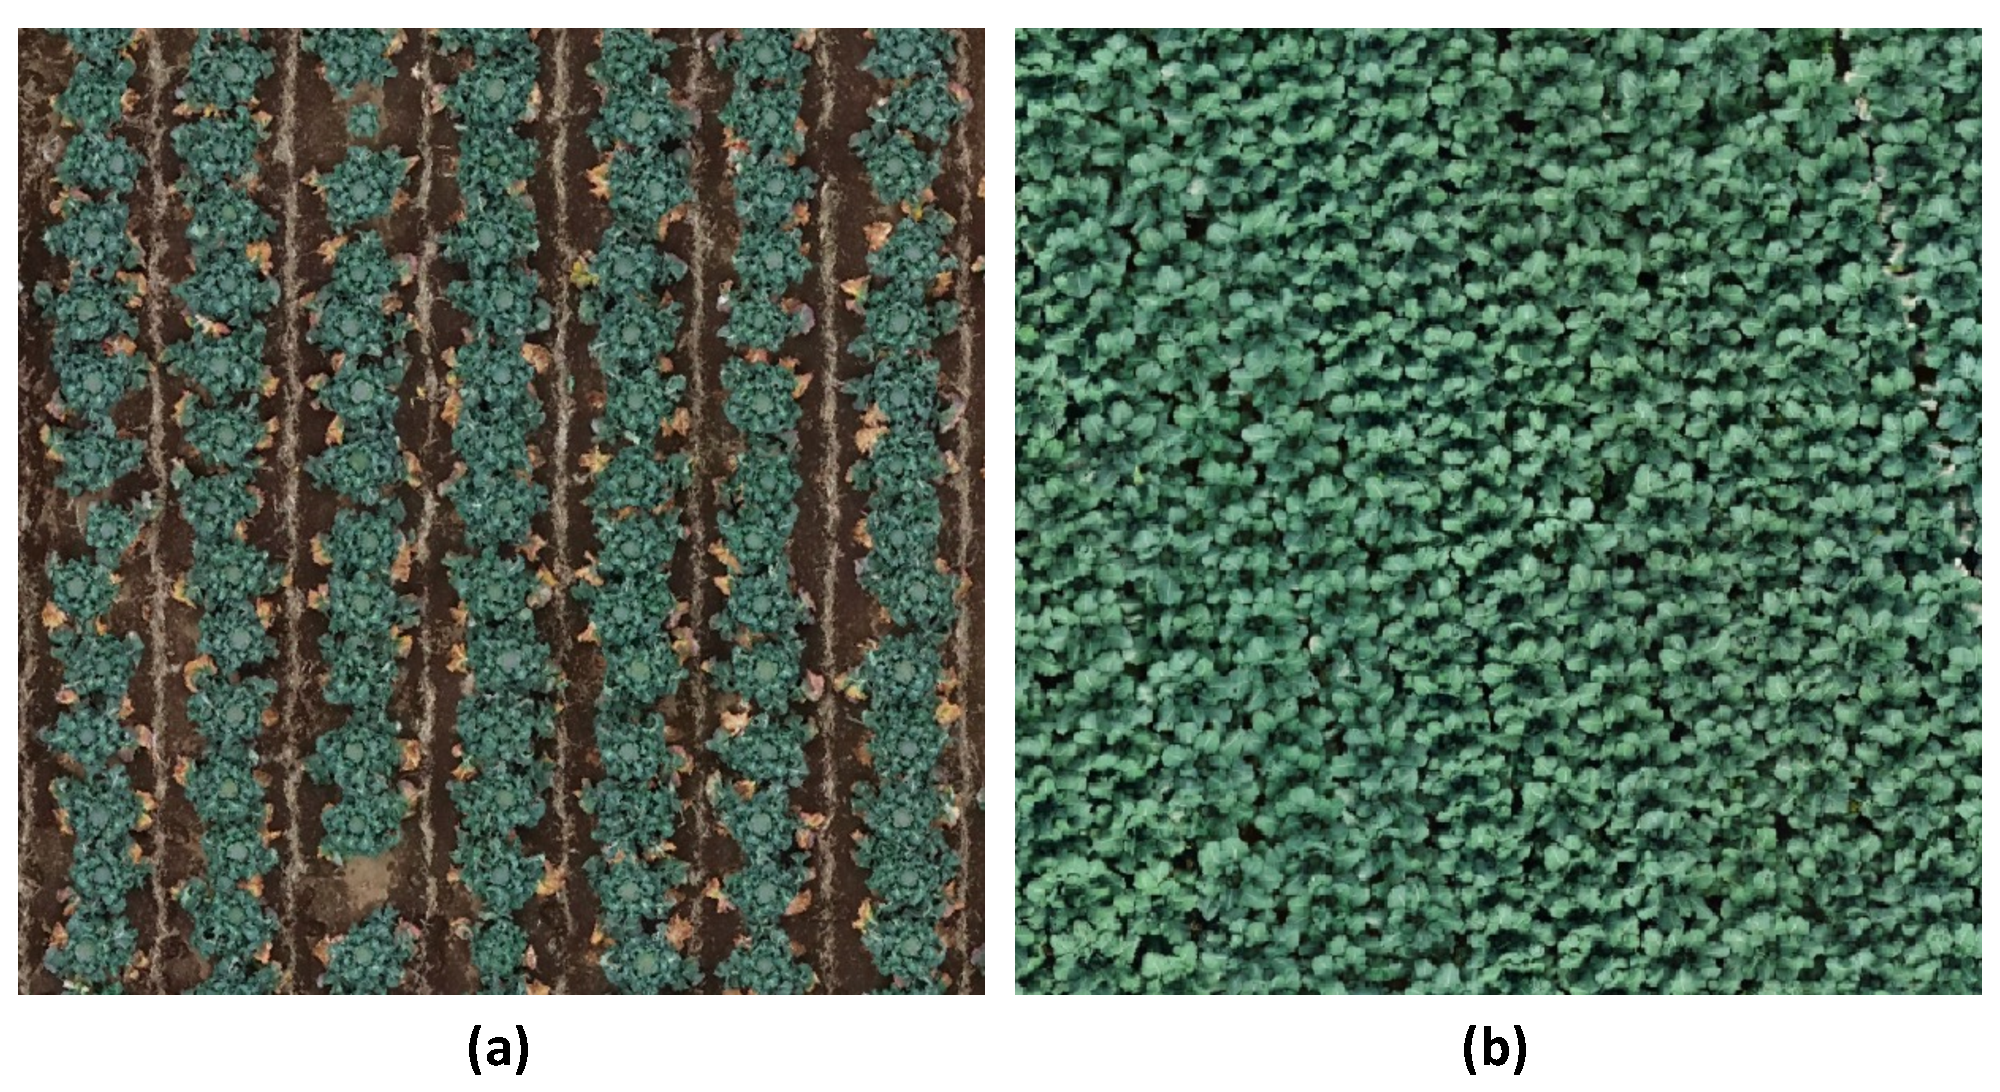
\includegraphics{figures/dis/pattern_diff.pdf}
    }
  \end{center}
  \caption[\added{The differences between the experimental field and actual farmland}]{
    \added{The differences between the experimental field and actual farmland. (a) is our experimental field in Tanashi of this study. (b) is a broccoli farmland in Fukushima from another project.}
  }
  \label{fig:dis_pattern}
\end{figure}

\added{
  Firstly, in Fukushima, the broccoli tends to have smaller leaf angles compared to the experimental fields. 
  This leads to the broccoli heads being heavily covered by the shadows of leaves. 
  These shadows create dark areas, making it challenging to visually identify the flower heads or leaves in the aerial images and also complicating the segmentation process. 
  To effectively address this issue, the utilization of advanced sensors such as multispectral or \gls{lidar} is warranted, but at a much higher cost as compared to the conventional RGB camera. Therefore, there is a need to develop a more cost-effective \gls{lidar} solution to cater to the future demands of farmland applications.
}

\added{
  Secondly, the closer row spacing and higher deviation make it infeasible to use our previous linear-based ridge detection algorithm. 
  Without it, assigning regular ID numbers to individual broccoli based on the order of the ridge becomes impractical.
  One potential approach is to abandon the use of sequential numbers for identification purposes along the ridges. 
  Instead, numbering can be determined based on the sorted XY coordinate positions. This alternative not only reduces the computational burden for ridge detection but also guarantees the uniqueness of the identification numbers. 
  However, this solution suffers from a disadvantage: 
  it becomes challenging to conveniently associate the numbers with the plants in the field. 
  Given that the actual measurements typically occur along the ridges, during recording, it becomes necessary to repeatedly verify the ID instead of simply incrementing it by 1 as in the previous solution.
  However, it is important to note that in the Fukushima farmland, conducting field measurements along ridges is not feasible. This issue will be discussed further in the upcoming point.
}

\added{
  Thirdly, the high planting density poses difficulties in sampling and field measurement.
  In Figure~\ref{fig:dis_pattern}.b, it is evident that the density of the actual farmland makes it difficult for people to enter without causing damage to the broccoli and soil. 
  However, the farmland owner does not allow such damage, leaving only the broccolis along the plot boundaries available for measuring and sampling. 
  Unfortunately, these boundary broccolis do not represent the same growing conditions as those in the plot center. 
  This poses a critical problem for the current pipeline since it leads to a lack of accurate ground truth data for model calibration.
  To address this issue in the future, a closer collaboration with more farmland owners is necessary. 
  For one thing, a carefully designed sampling strategy needs to be implemented before transplanting the broccoli. 
  For another, we can enlarge our broccoli database through such collaborations.
  We can potentially provide prediction services for farmlands where ground truth data is unavailable. 
  This can be achieved by identifying similar environmental and cultivar patterns already present in our database.
}

\subsection{\added{Lacking full participation}} \label{sec:lackdata}

\added{
  This is a personal limitation rather than the study itself.
  One thing that needs to be pointed out is I did not contribute entirely to the full process of the broccoli project. 
  The main focus of my doctoral research lies in the development of algorithms and engineering aspects. 
  Many in-field contributions were made by several collaborators.
  For example, the plant materials used in this study were provided by another student, \mbox{\citet{nishida_estimation_2023}}, in the laboratory. To be more specific, the experimental design of obtaining variate broccoli sizes by different fertilizations and the measurement of field data were primarily carried out by Nishida. 
  Meanwhile, the transplanting and daily field management of broccoli were conducted by technicians from ISAS.
  While the operation of the unmanned aerial vehicle (UAV) and data collection were mainly completed by Dr. Wei Guo.
  Additionally, I implemented some parts of the deep learning codes with the assistance of Tang Li from another laboratory. 
  With his assistance, I was able to apply deep learning methods to process certain data and provide technical reserves for subsequent engineering applications.
  Thanks to their help, I was able to focus my efforts on the engineering aspects of indoor reconstruction systems (Chapter 2), 
  the batch processing workflow of aerial data, and the accuracy improvement of spatiotemporal scale fusion (Chapter 3), 
  as well as the calibration, transformation, and matching of the broccoli model across different scales (Chapter 4).
  Such research experience has provided me with the opportunity to engage in interdisciplinary collaboration and have successfully achieved breakthroughs in my area of study. 
}

\added{
  However, this may not be beneficial to my overall academic development in some content. 
  Due to not being involved throughout the experimental process and data collection, it limits my understanding of the physiological and structural aspects of broccoli in the study. 
  It has made me aware of my shortcomings in research and motivated me to address them. 
  For example, during the period of broccoli transplanting, I visited the site several times to observe and inquire about the relevant details of plot settings. 
  When Nishida conducted field measurements and destructive sampling, I assisted with some measurements and destructive sampling work to gain insight into the details of field measurements. 
  Furthermore, when Dr. Wei Guo carried out drone data collection, I took the opportunity to learn the basic procedures of operating a drone and understood the effects of setting overlap, shutter speed, and exposure on the quality of photographs. 
  After this collaboration experience of my doctoral study, I have come to recognize the importance of actively participating in experiments and data collection for future research.
}

% \section{\added{Industry–Academia collaboration challenges}} \label{sec:appclg}

% \added{
%   In addition to the challenges and limitations inherent in this study, the practical application of similar smart agriculture research also presents its own set of limitations and challenges. 
% }


\section{Future research prospects} \label{sec:respros}

In this thesis, several new approaches or pipelines were proposed to \replaced{enhance the performance of 3D-based plant phenotyping. 
While our experimental field exhibits promising results, as discussed previously, this study still faces unresolved limitations at its current stage. 
In this section, I will explore the future research prospects that not only benefit this study but also inspire further advancements in smart agriculture.}
{improve the performance of 3D-based plant phenotyping. It was suggested to extend each of them in the future. As mentioned in Chapter 2, the dual-rotation approach for data collection still needs manually change and vertically flip plants, and only applicable to solid plants. A more automated instrument should be developed to further reduce manual operations. For example, by using a track controlled by a stepper motor or robotic arms to achieve automated plant replacement and rotation. For softer plant organs like leaves and flowers, the dual-rotation method may not work due to the structure changing, so the approach needs to be changed by setting up camera arrays at different angles to achieve similar results.
}

\subsection{\added{Probabilistic of this study}}

\added{
  Although our current research has some shortcomings and limitations, 
  a set of tools and pipelines we developed in this study has been helping many subsequent research projects, 
  not only limited to the agricultural field.
}

\added{
  Chapter 2 presents the establishment of high-quality close-range crop modeling pipelines.
  We obtained 189 high-resolution 3D models of broccoli plants through it. 
  As mentioned previously, this workflow can be readily extended to modeling more similar crops, including potatoes, sweet potatoes, and various other fruits.
  These high-quality 3D plant organ models can subsequently undergo phenotypic analysis. 
  Moreover, our 3D database holds potential for application in the \gls{cg} or gaming industry, as it offers high-resolution assets for use in AAA games.
}

\added{
  As a dependency tool to Chapter 3, 
  we first developed an Intermediate Data Processing (IDP) tool, named EasyIDP \mbox{\citep{wang_easyidp_2021}}, 
  to address the issue of low quality of drone-based 3D reconstruction outputs. 
  This tool not only found good application in our third chapter but has also been applied and highly praised in other industries that require the use of drone measurement. 
  For example, Prof. Benjamin Weinstein, from the University of Florida, used our tool for avian ecology surveys; 
  Prof. Derek Young, from the University of California Davis, used our tool for optimizing forest species research; and
  Engineer K. Senda, from the Japanese company Yumeni, used our tool for improving urban greening monitoring. 
  As of September 2023, our GitHub project community (\url{https://github.com/UTokyo-FieldPhenomics-Lab/EasyIDP}) has received 34 stars and 22 discussion threads. 
  We have established a positive open-source community feedback mechanism,
  which is a level of achievement that other similar researchers have not reached. 
  It is important to further improve and promote these types of open-source software and communities in order to ensure the reproducibility and contribution of our work.
}

\added{
  In Chapter 3, an improved aerial survey pipeline for broccoli size was established, 
  which obtained the specific size of each broccoli plant in the time series. 
  This is difficult to achieve with traditional methods in acceptable labor costs. 
  Subsequently, other members of the laboratory based on this technology, combined with meteorological data and growing degree models, 
  successfully developed an individual-based broccoli growth prediction method \mbox{\citep{wang_drone-based_2023}}. 
  It was also found that the deviation of only 2 days from the optimal date, 
  The profit difference in one hectare of the experimental field could reach \$2000, 
  indicating significant implications for reducing food loss and improving farmers' income \mbox{\citep{wang_drone-based_2023}}. 
  Although it currently cannot be directly applied to densely planted farmlands, 
  with the subsequent integration of other sensors to solve the broccoli segmentation problem, this process can be smoothly applied.
}

\added{
  Chapter 4 uses data fusion to achieve a better visualization effect, 
  transforming numerical phenotype data (such as broccoli size) into a 3D intuitive model. 
  This also serves as the technical basis for subsequent digital twins and smart agriculture, which is further discussed in Section~\ref{sec:digitwin}. 
  If \gls{ar} and \gls{vr} technologies can be combined in the future, 
  there is hope to transform the laborious field patrol work into indoor activities. 
}


\subsection{\added{Probabilistic of 3D reconstruction}}

\added{
  The study primarily utilizes photo-based 3D reconstruction (\mbox{\gls{sfm}-\gls{mvs}}) to acquire 3D data for both close-range and aerial plants. 
  In comparison to other reconstruction methods (Figure~\ref{fig:int2}), \mbox{\gls{sfm}-\gls{mvs}} offers the key advantage of relatively low sensor costs. 
  Only common RGB cameras are necessary to yield satisfactory results for close-range or aerial reconstructions.
  However, the workflow of photo-based 3D reconstruction also presents several challenges for data management and processing algorithms that deserve to be considered for future research.
}

\added{
  The first point is about data storage and management. 
  Typically, modeling a scene requires a large number of images, which can occupy a minimum of 1GB of storage space. 
  In our 3-year study, for both close-range broccoli head modeling (Chapter 2) and aerial survey (Chapter 3), the raw image data reached over 350GB 
  (135GB in 2020, 30.3GB in 2021, and 101.7GB in 2022 for aerial survey; 87GB for close-range modeling). 
  Furthermore, the data size from data preprocessing, reconstruction process, and the resulting model is essentially the same as the raw image data. 
  This amount of data is only applicable to a 1-hectare experimental field, and the volume of data increases proportionally with the area. 
  While it is theoretically possible to delete the original data and intermediate processes after obtaining the final modeling results to free up space, this is not feasible for our pipeline. 
  We need to merge the final results with the raw images to achieve more accurate segmentation results. 
  Additionally, these raw data hold significant value as digital resources for smart agriculture research. 
  When properly preserved, they can serve multiple research groups in answering complementary research questions over the years \mbox{\citep{guo_uas_2021}}. 
  Therefore, compared to using local hard drives for data storage and archiving, the use of centralized cloud storage not only ensures better data security but also enables fast data sharing across institutions. 
  This is a crucial aspect that smart agriculture must consider for future data storage and management \mbox{\citep{guo_uas_2021}}. 
  Simultaneously, it is imperative to collaborate with various research institutions to establish a unified data archiving and metadata storage standard, similar to that of meteorological data, for subsequent cross-regional and long-term research tracking.
}

% However, 
%    rather than plants, particularly under natural field conditions. 
%   The complex combination of lighting, temperature, and humidity in the field, along with the presence of weeds, wind turbulence, and occlusions, present significant challenges for image-based 3D reconstruction.
%   Hence, 

% Nonetheless, it should be noted that this algorithm assumes the reconstructed object to be rigid and may not be universally applicable to all agricultural crops. To evaluate its feasibility, we selected broccoli, which closely resembles a rigid body, as the subject for our case study. Even so, attaining optimal data quality while controlling expenses still requires a substantial amount of effort.

\added{
  The second point concerns the processing algorithm of 3D reconstruction.
  It should be noted that this algorithm assumes the object to be rigid and consistent throughout all points of view (photos). 
  This assumption is commonly valid for urban buildings, mine shafts, and cultural relics,
  rather than capturing dynamic objects (such as those affected by wind-induced movement), 
  repeatable structures (such as similar plants in a field), 
  and reflective objects (for instance, paddy fields). 
  These cases commonly arise in agricultural applications, and additionally along with complex combinations of lighting, humidity (cloud and fog),  presence of weeds, and occlusions.
  Several studies have been conducted to address the challenges posed by complex situations in algorithm adaptation. 
  For instance, \mbox{\citet{zheng_sparse_2015}} focused on enhancing the reconstruction effect of dynamic components through algorithmic improvements. 
  However, it is not feasible to manually develop special algorithms for all different kinds of natural conditions, a more efficient and robust approach should be found.
}

\added{
  The potential application of deep learning technology to partially or entirely replace the SfM-MVS algorithm has also raised many research interests \mbox{\citep{li_dl-based_2022}}. 
  This includes the substitution of camera pose estimation, also known as bundle adjustment \mbox{\citep{vedaldi_deepsfm_2020}}, and point cloud densitification \mbox{\citep{ferrari_mvsnet_2018}}. Furthermore, the \gls{nerf} builds upon the outcomes of the \gls{sfm} algorithm and employs deep learning networks to supplant subsequent \gls{mvs} and 3D object generation processes \mbox{\citep{mildenhall_nerf_2022}}. For example, \mbox{\citet{jignasu_plant_2023}} successfully achieved excellent reconstruction outcomes for maize, underscoring the effectiveness of this approach.
}% nerf app
\deleted{In addition, besides image-based photogrammetry, the latest \gls{nerf} technology is also worth exploring.} There is now an application of \gls{nerf} based on the latest iPad's \gls{lidar} sensor for camera position estimation. In our preliminary experiments in early May 2023, especially for landscape plants with complex structures, better 3D models can be obtained than with photogrammetry. However, currently, the iPad needs to be manually moved to match the path guidance in the software. If this process can be interactively realized with a robotic arm, it also has broad potential applications.

\added{
  In addition to enhancing the \gls{sfm}-\gls{mvs} workflow, there have been studies exploring the utilization of deep learning for direct 3D structure prediction. 
  For instance, \mbox{\citet{vicini_differentiable_2022}} employ direct estimation to determine the 3D shape, while \mbox{\citet{magistri_towards_2021}} utilize a single image in conjunction with deep learning to directly render the 3D plant model. 
  These studies, based on deep learning techniques, aim to overcome the technical limitations associated with conventional 3D reconstruction algorithms. 
  It is important to verify and implement these approaches in the acquisition of 3D plant structures in the future.
}

\added{
  The third point is about multi-sensor integration. 
  The aforementioned attempts to reconstruct 3D structures from photos and optimize various algorithms are compromised solutions due to equipment costs. 
  However, if we neglect equipment costs, the use of \gls{lidar} is a more accurate method of obtaining spatial 3D structures. 
  \gls{lidar} has been extensively applied and tested in both close-range and outdoor studies \mbox{\citep{thapa_novel_2018,lin_segmentation_2022,jin_lidar_2021}}. 
  With the continuous development of autonomous driving and sensor technology, 
  the price of \gls{lidar} is continuously decreasing \mbox{\citep{ackerman_lidar_2016}}. 
  It is expected that within the next 10 years, 
  the price of \gls{lidar} will approach that of advanced \gls{dslr} cameras, 
  potentially revolutionizing the acquisition of 3D structural data. 
  In terms of applications in smart agriculture in the future, 
  the fusion of \gls{lidar} with other sensors further enhances the performance of high-throughput models \mbox{\citep{li_multi-source_2023,nguyen_uav_2023}}.
}

\added{
  The final point is regarding the automation technologies utilized in aerial data collection. 
  Presently, the quality of aerial image data still greatly depends on the expertise of device operators. 
  Due to varying weather conditions during different survey times, 
  there are currently no universal settings that are suitable for all conditions. 
  Consequently, operators must manually adjust camera settings, 
  such as exposures and shutter speed, according to the prevailing weather conditions. 
  However, these adjustments heavily rely on experience, 
  which encompasses not only drone operation but also a profound understanding of post-data processing. 
  Often, the data collection work is outsourced to technicians or personnel from other institutions working remotely, 
  and its quality frequently proves challenging to meet the high-precision analysis requirements.
  The implementation of this personnel training approach is not feasible. 
  Instead, it is necessary to establish collaboration with drone companies to develop a camera mode, 
  which can automatically adjust based on the surrounding environment for effective agricultural data collection. 
  This approach will diminish the requirement for personnel expertise. 
  This has already been demonstrated in previous technological advancements. 
  Initially, manual control the drone flight and camera photography was essential during aerial surveys around the 2010s. 
  However, the acquired images often failed to meet the required level of overlap, resulting in reconstruction failure. 
  Consequently, when I attended the internship at the Chinese Academy of Forestry, 
  we developed the software for flight route control with required overlaps \mbox{\citep[\url{www.uav-hirap.org}]{wang_uav-hirap_2017}}. 
  These features allow for automatic flight route planning on a computer and transmitting to the drone. 
  This technology has since been completely superseded by the built-in flight planning function of drones within three years. 
  Hence, it can be predicted that this issue of camera parameter settings will also be integrated into drones shortly to ensure the stability of data quality obtained by different operators.
}

\subsection{\added{Probabilistic of digital twin}}\label{sec:digitwin}

\added{
  The advent of digital twin technology points to a very different future for smart agriculture and plant phenotyping, 
  the researchers can operate directly on the virtual plants and preview its impact on the plant immediately \mbox{\citep{verdouw_digital_2021}}. 
  The fundamental in implementing such technology is to present the 3D crop model (virtual plant) accurately in the computer first, and then implement architecture fine-tuning and phenotyping applications on them.
  This study is the first to explore the possibility of presenting the virtual plants from actual fields accurately.
}

% Virtual plants powered crop data analysis and phenotyping applications.
In Chapter 4, the data fusion between close-range and aerial surveys showed a good result in the visualization hidden part of the broccoli head, although based on statistical regression for visualization rather than actual status. As discussed in Chapter 4, for different cultivars of broccoli, more broccoli heads should be collected to provide a sufficient template database to meet more detailed transformation needs. However, the proposed method is facing challenges when dealing with crops with complex structures, such as maize or soybean canopies. On one hand, the severity of occlusion makes it very difficult to distinguish individual maize or soybean; on the other hand, due to the multilateral structure of crops, it is difficult to collect enough samples for template transformation. \added{Thus, there is a demand to change the virtual plant architecture with lower cost} 

\added{
  Currently, there are three main methods of acquiring virtual plant that can be architecture fine-tuned. 
  1) By template stitching. 
  \mbox{\citet{chang_3dcap_2022}} obtained the database of wheat organ 3D models at different growth stages by destructive sampling and manual measurement of parameters. 
  Then combine those organs to one wheat by random picking and placing with random position angles within the range obtained by real measurements. 
  \mbox{\citet{wen_3d_2021}} applied the similar idea for maize. 
  2) By static deformation. 
  The 3D static model of whole maize (in point cloud format) was obtained by 3D reconstruction. 
  The maize model was then automatically segmented into organs, 
  and these segmented parts were transformed by applying geometric transformations to implement changes in architecture \mbox{\citet{liu_canopy_2021}}. 
  3) By parametric approximation. 
  The L-system was used to construct a parameter-adjustable virtual crop model and then adjusted the parameters to approximate the real crop by three-view photos \mbox{\citet{cieslak_l-system_2021}}. 
  % This process was also reflected in the implementation of \gls{cg} modeling. 
  % For example, the general shape of the plant was obtained through relatively simple geometries, 
  % and then photo-quality texture mapping was used to obtain a very realistic \gls{cg} model \mbox{\citet{mikami_hidden_2022}}.
}

\deleted{
In this condition, the advent of procedural modeling points to very different solutions which use several parameters to control the structure of 3D models. For example, The L-system was used to construct virtual crop models that adjusted the parameters to approximate the real crop by three-view photos \mbox{\citep{cieslak_l-system_2021}}.}
Although the model obtained using the above method is only structural, it is not realistic enough in terms of detail and appearance. \citet{mikami_hidden_2022} used photo-quality texture mapping on the plant 3D models with relatively simple geometries and finally obtained very realistic 3D models in texture. In our preliminary experiment, a similar corn model using parameter controls has already been achieved in Blender, but due to the complexity of the research, the ability to repair the corn canopy has not yet been realized. In subsequent studies, we hope to develop a parameter-controlled broccoli model and complete the repair of the corn canopy.

Furthermore, several advanced \replaced{techniques}{phenotyping applications} can be \replaced{applied to}{simulated on} the abovementioned virtual 3D plant models. 1) The ray-tracing technologies can be applied to simulate lights within the canopy. 2) The point cloud simulation technology can be used to simulate point clouds from the virtual canopy. For the canopy traits which are easy to get from virtual plants but hard from the real field, the corresponding models between features from the simulated point cloud and traits from the virtual canopy can be trained and then applied to the field-scanned point cloud data to inverse the actual data \citep{liu_estimating_2017}. 3) The \gls{cg} rendering techniques can decrease the workload of data annotating in the phenotyping data processing by deep learning. The rending engine can yield \gls{cg} photos that are very close to the real world. At the same time, by adjusting the model texture to solid pure color, the corresponding labeled information for both \gls{cg} photos \citep{mikami_hidden_2022} and point clouds \citep{chaudhury_3d_2020} can be generated in batch from random virtual canopies.

\subsection{\added{Probabilistic of large AI models}}

% current AutoML not working